\documentclass[11pt]{article}

\usepackage[a4paper,margin=1in]{geometry}
\usepackage{amsmath,amssymb,amsfonts}
\usepackage{booktabs}
\usepackage{longtable}
\usepackage{array}
\usepackage{graphicx}
\usepackage{xcolor}
\usepackage{hyperref}
\usepackage{enumitem}
\usepackage{caption}
\usepackage{float}

\graphicspath{{../figures/}}

\hypersetup{
  colorlinks=true,
  linkcolor=blue!50!black,
  citecolor=blue!50!black,
  urlcolor=blue!50!black
}

\newcommand{\R}{\mathbb{R}}
\newcommand{\V}{\mathcal{V}}
\newcommand{\E}{\mathcal{E}}
\newcommand{\WCA}{\mathrm{WCA}}
\newcommand{\diag}{\operatorname{diag}}
\newcommand{\MSE}{\operatorname{MSE}}

\title{\textbf{World Cellular Automata}\\
\large A Recursive Local-World Architecture for World-State Modeling\\
\normalsize Technical Report v0.1}
\author{WCA Research Project}
\date{2026-07-01}

\begin{document}
\maketitle

\begin{abstract}
World Cellular Automata (WCA) is a recursive architecture for world-state
modeling. Instead of mapping an observed state directly to a future state, WCA
expands a global state into a family of node-centered local worlds, evolves
those local worlds through learned pair interactions, and recomposes their
centers into the next global state. We develop the WCA architecture from its
finite-set and tensor semantics to a staged experimental program across mazes,
WeatherBench-style fields, and PDEBench reaction-diffusion. The central claim is architecture-first: recursive
local-world synthesis is a viable and testable primitive for structured
world-state prediction. The current evidence is strongest in token-level
PDEBench reaction-diffusion, where recursion depth, learnable field interfaces,
attribution controls, and h8x2 rollout diagnostics indicate that the WCA core
can contribute beyond interface-only and no-recursion alternatives. The report
also records negative results and unresolved boundaries, including larger-token
PatchMean underperformance, native-resolution visual limits, and systems
scaling constraints. These limitations are not treated as failures of the
research direction, but as the next experimental frontier.
\end{abstract}

\tableofcontents
\newpage

\section{Scope and Use}

This release is written as a complete research record rather than a compressed
conference submission. Its purpose is to make the WCA program legible and
reproducible: what the architecture is, why it is worth studying, what has
been tested, what the experiments show, what they do not yet show, and which
next steps are scientifically justified.

The report is intended for public release on GitHub, Hugging Face, and Zenodo.
It therefore favors completeness over page economy. It includes architecture
motivation, mathematical notation, shape contracts, experimental protocol,
selected results, negative findings, and a roadmap. Traditional algorithm-box
pseudocode is intentionally omitted. WCA is not best understood as a generic
training loop. Its important property is the semantic structure of the
intermediate local-world tensor and the preservation of the center index during
pair evolution.

\section{Why Study WCA?}

Physical and embodied prediction tasks require both local interaction and
global coherence. Reaction-diffusion, contact dynamics, heat transfer,
shortest-path navigation, and weather fields all involve local rules whose
effects accumulate into global states. A model that treats the future as a
single direct output can perform well, but it often hides the mechanism of state
evolution inside a black-box map. A purely local cellular automaton has a clear
mechanism, but it can struggle to retain global context over long horizons.

WCA proposes a middle path. Each node is allowed to construct a local
interpretation of the entire world, evolve that local world through pairwise
relations, and then contribute its evolved center back to the shared world
state. This gives the model a concrete recurrent structure:

\[
H_t \longrightarrow L_t \longrightarrow L'_t \longrightarrow H_{t+1}.
\]

The motivation is not only empirical. WCA is attractive because it makes a
specific architectural wager:

\begin{quote}
World-state prediction can be improved by repeatedly differentiating a global
state into node-centered local worlds and recomposing those evolved local
worlds into a shared next state.
\end{quote}

This wager is falsifiable. If recursion depth does not matter, if no-recursion
controls match the full core, if tokenizer-only controls explain the gain, or
if long-horizon rollout collapses, then the WCA hypothesis weakens. The
experiments in this report are organized around these tests.

\section{Mathematical Formulation}

\subsection{World state}

Let the represented world have a finite node set

\[
\V = \{1,2,\ldots,N\}.
\]

At time $t$, WCA represents the world as a hidden state function

\[
h_t:\V \rightarrow \R^D,
\]

or, in batched tensor form,

\[
H_t \in \R^{B \times N \times D},
\]

where $B$ is batch size, $N$ is the number of nodes or field tokens, and $D$ is
the hidden dimension.

\subsection{Local worlds}

The defining move of WCA is to expand the world state into a family of local
worlds:

\[
L_t = \Pi_\theta(H_t), \qquad
L_t \in \R^{B \times N_c \times N_v \times D}.
\]

In the protected dense baseline, $N_c=N_v=N$. The first node axis indexes the
center $c$ of a local world. The second node axis indexes the represented world
node $r$ inside that centered world. In function notation, a local world is

\[
\ell_{t,c}: \V \rightarrow \R^D,
\]

and the full bundle of local worlds is

\[
\{\ell_{t,c}\}_{c\in \V}.
\]

This is the key distinction from ordinary message passing. WCA does not only
update $h_t(i)$ from neighbors of $i$. It constructs a center-indexed family of
world interpretations and evolves each interpretation before recomposition.

\subsection{Pair evolution inside local worlds}

Inside a local world centered at $c$, WCA evolves receiver node $r$ by
aggregating pair interactions with sender nodes $s$:

\[
\ell^{k+1}_{t,c}(r)
=
\ell^{k}_{t,c}(r)
+
\sum_{s\in \V}
A_{rs}\,
\phi_\theta
\left(
\ell^{k}_{t,c}(r),
\ell^{k}_{t,c}(s),
e_{rs}
\right).
\]

Here $A_{rs}$ is a support or adjacency weight, $e_{rs}$ is optional edge
information, $\phi_\theta$ is a learned pair kernel, and $k$ indexes inner
pair-evolution steps. The full dense semantics are equivalent to an interaction
over

\[
(b,c,r,s,d) \in
\{1,\ldots,B\}\times \V \times \V \times \V \times \{1,\ldots,D\},
\]

which has semantic shape

\[
[B,N,N,N,D].
\]

Implementations may chunk or reorder computation for memory, but the protected
baseline claim depends on preserving this semantic structure.

\subsection{Center recomposition}

After $K$ inner pair-evolution steps, WCA recomposes the next world state from
the evolved center diagonal:

\[
h_{t+1}(i)
=
\rho_\theta\left(\ell^{K}_{t,i}(i)\right),
\]

or, in tensor shorthand,

\[
H_{t+1}
=
\rho_\theta\left(\diag L_t^K\right).
\]

The center index is therefore not an implementation accident. It is a semantic
carrier. The local world centered at $i$ contributes the evolved representation
of node $i$ to the next global state.

\subsection{Outer recursion}

The previous definition gives one outer update. WCA can apply the update
multiple times:

\[
H_{t}^{(m+1)}
=
F_\theta\left(H_t^{(m)}, A, E\right),
\qquad
m=0,\ldots,M-1.
\]

The final prediction is read from $H_t^{(M)}$. In the experiments, $M$ is
called outer recursion depth. The V25 recursion-depth ladder tests whether
larger $M$ improves long-horizon physical prediction.

\section{Shape Contract and Architecture Invariants}

\begin{longtable}{p{0.22\linewidth}p{0.26\linewidth}p{0.42\linewidth}}
\toprule
Object & Shape & Meaning \\
\midrule
$H_t$ & $[B,N,D]$ & Global world state at time $t$. \\
$L_t$ & $[B,N,N,D]$ & Center-indexed local-world bundle. \\
Pair semantics & $[B,N,N,N,D]$ & Batch, center, receiver, sender, channel. \\
$\diag L_t$ & $[B,N,D]$ & Evolved centers used for recomposition. \\
$H_{t+1}$ & $[B,N,D]$ & Next global world state. \\
\bottomrule
\end{longtable}

The protected WCA baseline must preserve the following invariants:

\begin{enumerate}[leftmargin=2em]
  \item The model maintains a world state $H_t\in\R^{B\times N\times D}$.
  \item The model constructs local worlds $L_t\in\R^{B\times N\times N\times D}$.
  \item Pair evolution acts inside local worlds and preserves the center index.
  \item Recomposition extracts evolved centers into $H_{t+1}$.
  \item Memory optimization must preserve dense semantics unless declared as an explicit variant.
\end{enumerate}

\begin{figure}[H]
\centering
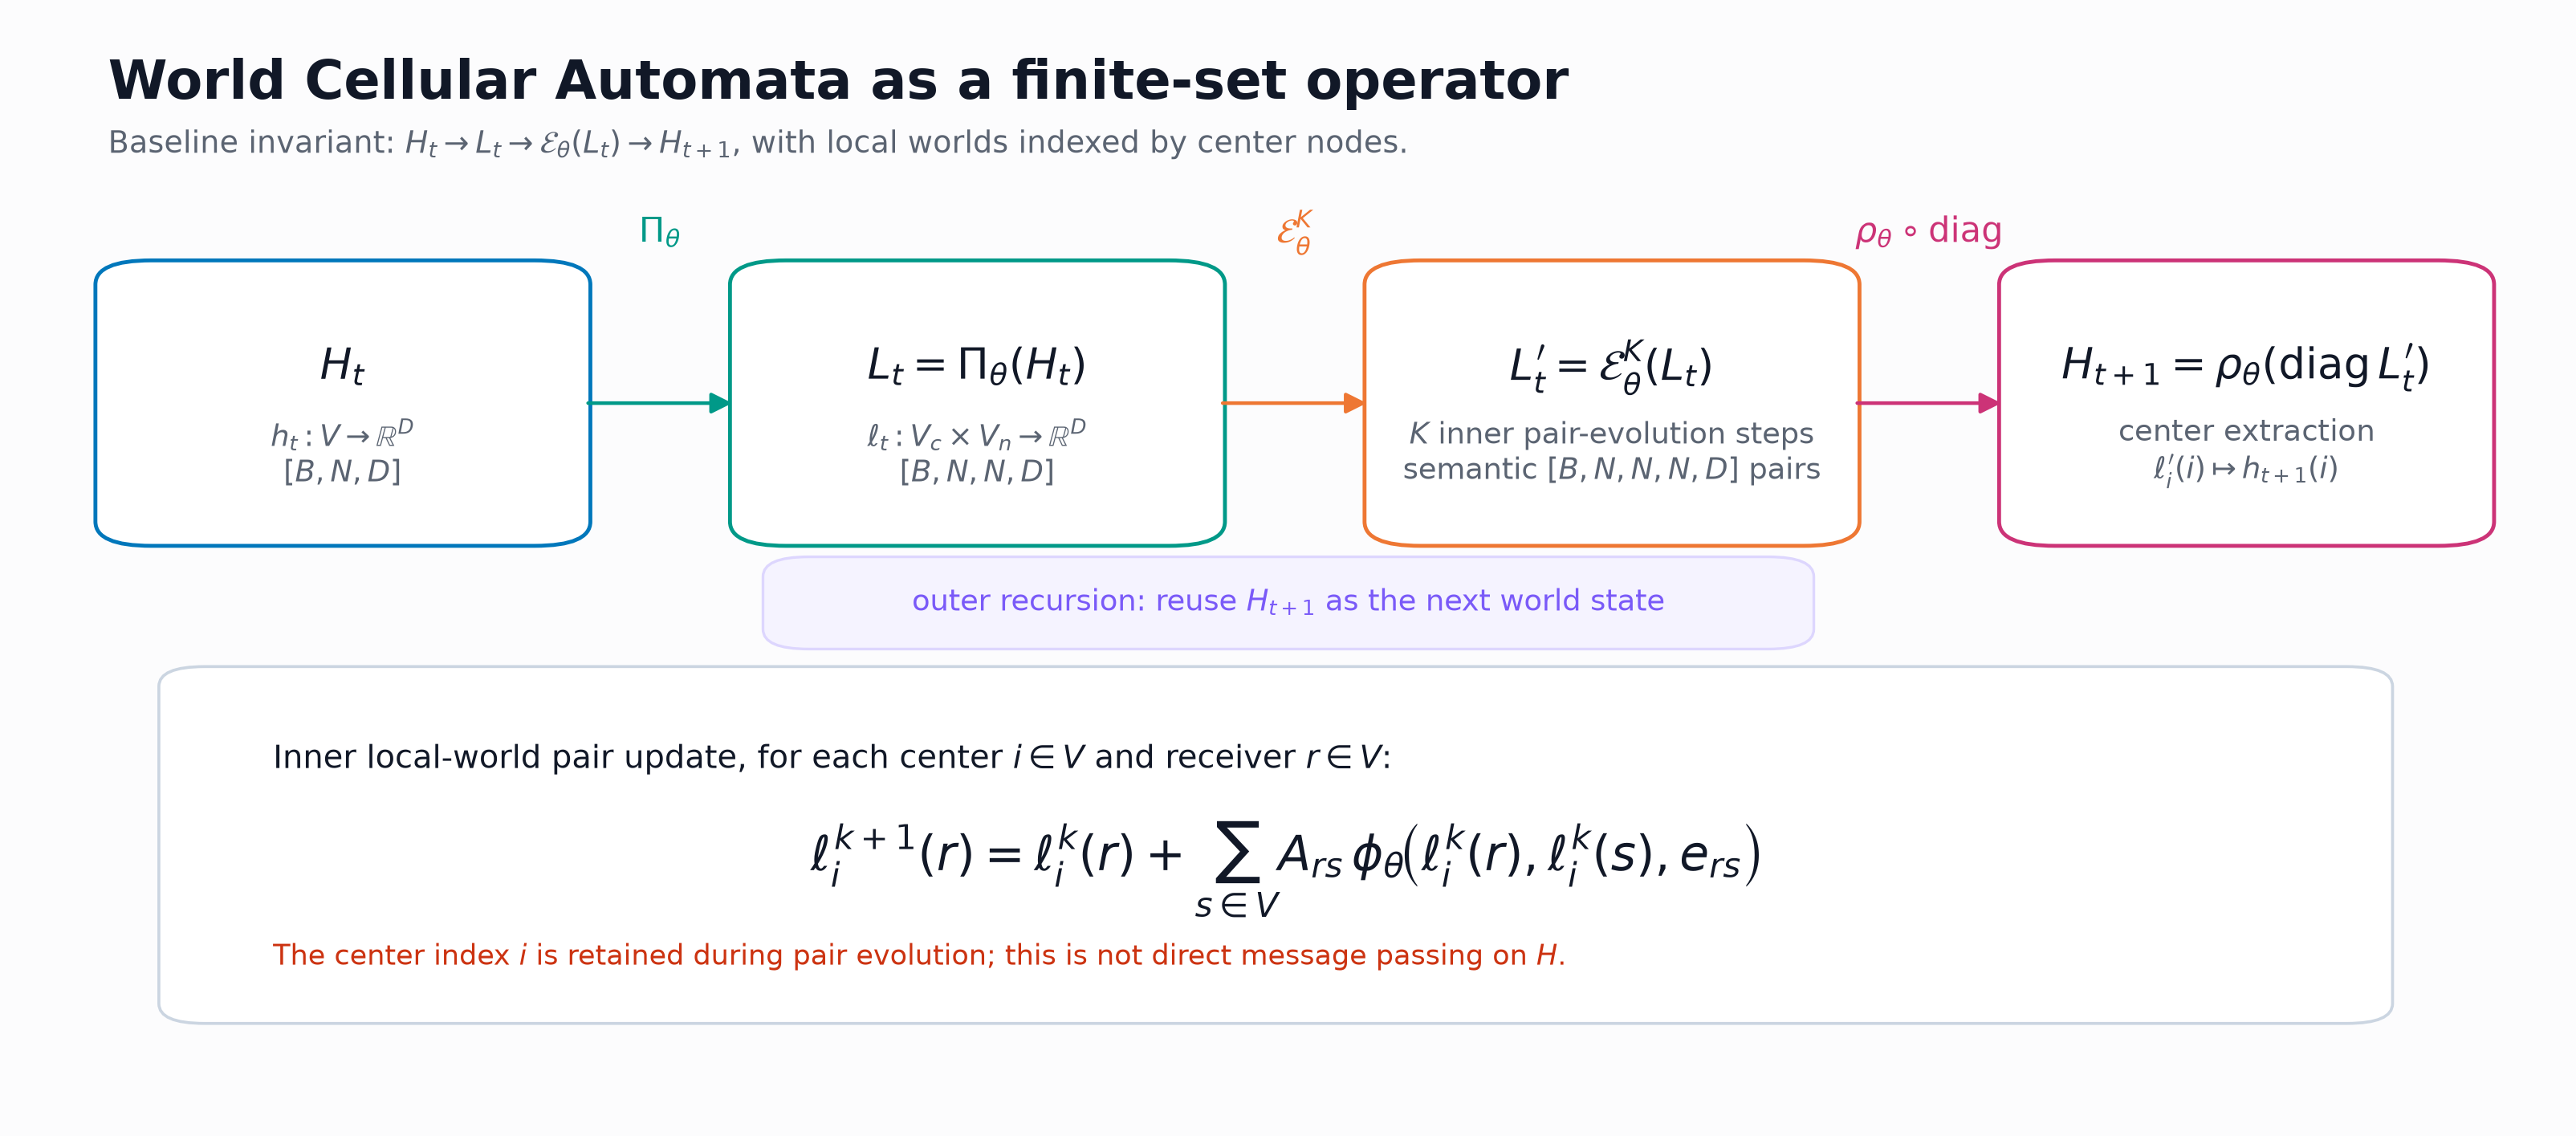
\includegraphics[width=0.95\linewidth]{wca_formal_operator_diagram.png}
\caption{WCA as a finite-set operator. The protected semantic invariant is
$H_t \rightarrow L_t \rightarrow \mathcal{E}_\theta(L_t) \rightarrow H_{t+1}$.
The key intermediate object is the center-indexed bundle of local worlds.}
\end{figure}

\begin{figure}[H]
\centering
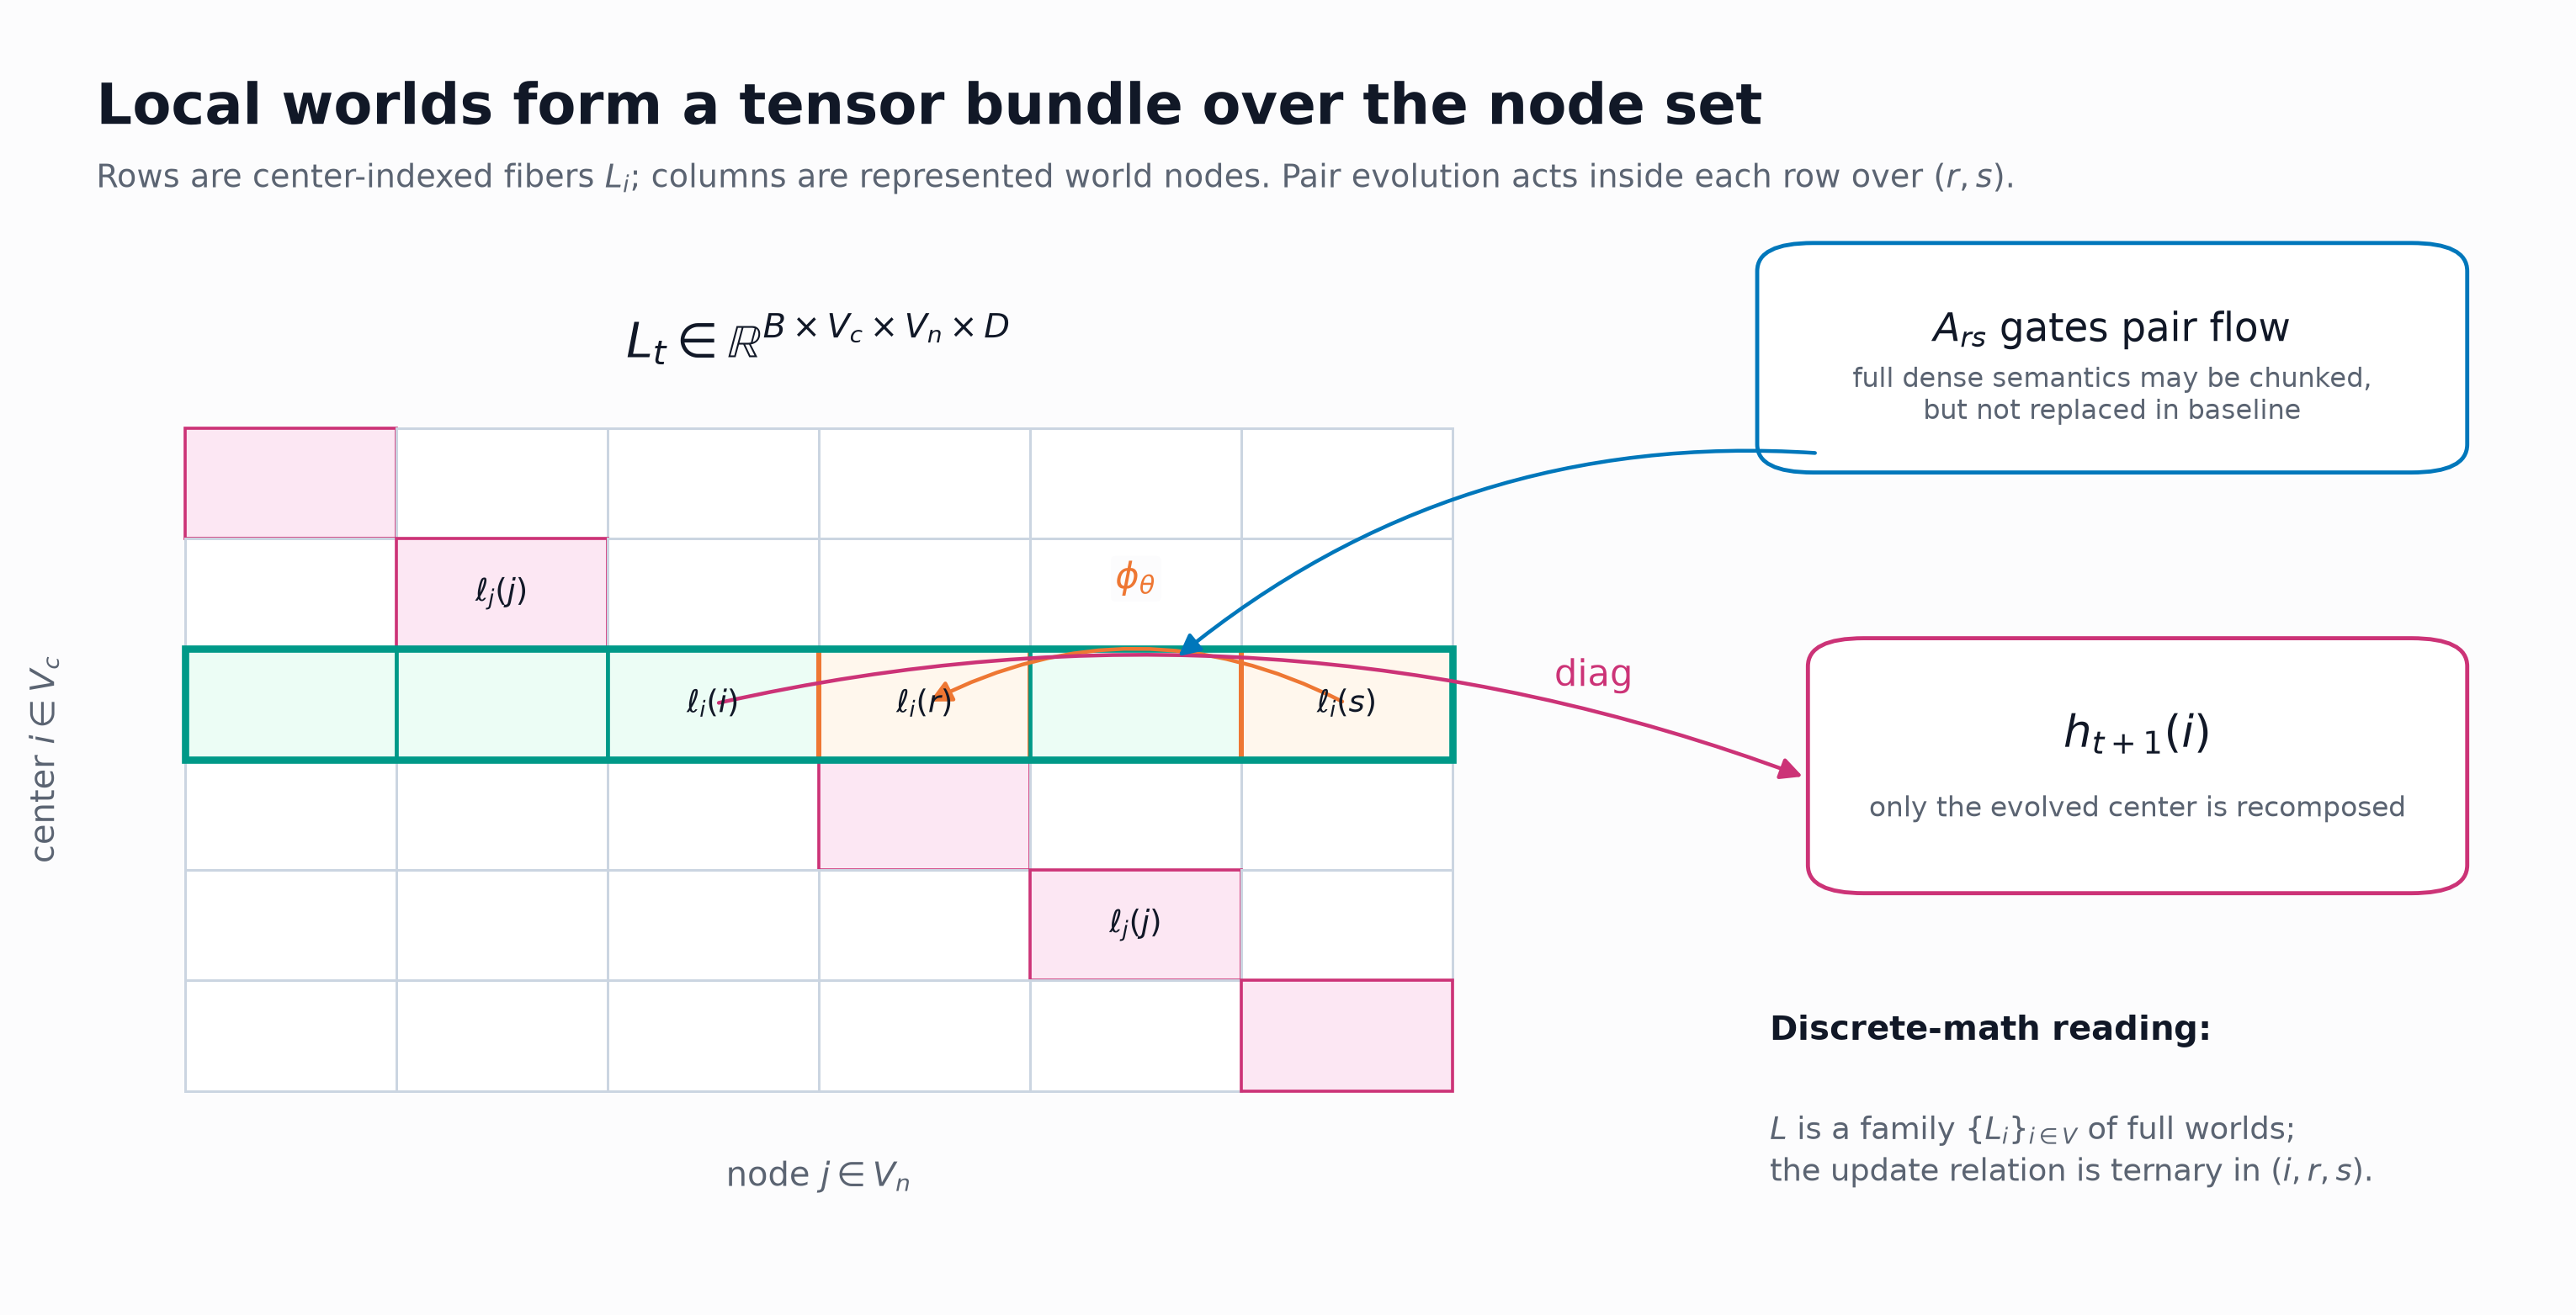
\includegraphics[width=0.95\linewidth]{wca_formal_tensor_fiber_diagram.png}
\caption{Local worlds form a tensor bundle over the node set. Pair evolution
acts inside a row indexed by center $c$ over receiver and sender positions
$(r,s)$; recomposition uses the evolved diagonal.}
\end{figure}

\section{Relation to Other Model Families}

\subsection{Versus neural cellular automata}

Neural Cellular Automata learn local update rules over grid states. WCA shares
the intuition that repeated local transformations can produce global structure,
but WCA is not only a local grid rule. Each center $c$ carries a local world
$\ell_c$ over the full represented node set. The update is therefore a
local-world evolution, not simply a neighborhood update around one grid cell.

\subsection{Versus graph neural networks}

A message-passing GNN typically updates node $i$ using messages from neighboring
nodes $j$:

\[
h_{i}^{+}
=
\psi_\theta
\left(
h_i,
\sum_{j\in \mathcal{N}(i)}
\phi_\theta(h_i,h_j,e_{ij})
\right).
\]

WCA instead evolves $\ell_c(r)$ inside every center-indexed local world:

\[
\ell_c(r)^{+}
=
\ell_c(r)
+
\sum_s A_{rs}\phi_\theta(\ell_c(r),\ell_c(s),e_{rs}).
\]

The additional center index $c$ is the architectural difference. Removing it
collapses WCA toward ordinary graph message passing and must be treated as an
ablation, not as an equivalent implementation.

\subsection{Versus transformer attention}

Transformer attention computes data-dependent weighted interactions among
tokens. WCA also learns relations among nodes, but it does not rely on a
standard query-key-value attention block. Its distinctive structure is the
creation, evolution, and recomposition of local worlds. Attention could be used
inside a future pair kernel variant, but that would be a variant of WCA, not the
protected baseline described here.

\subsection{Versus neural operators}

Neural operators learn maps between function spaces. They are strong baselines
for PDE surrogate modeling because they can efficiently map present fields to
future fields. WCA asks a different question: can a recursive state machine
over local-world bundles learn useful world dynamics? The comparison is not
``WCA replaces FNO.'' The comparison is whether WCA provides a distinct
architecture primitive that can be controlled, attributed, scaled, and combined
with future interfaces.

\section{Interfaces: From Fields and Mazes to World Tokens}

WCA consumes vectorized state tokens. It does not currently consume text tokens
in the language-model sense. A field, maze, or future multimodal state must be
mapped into $H_t$.

\subsection{Maze interface}

For a maze, the node set $\V$ corresponds to grid cells. Input channels include
wall, start, goal, coordinates, and open-cell indicators. The output is a
potential or distance-like field used for greedy navigation. The functional
metric is not just field MSE; a useful maze field must support path rollout
from start to goal.

\subsection{PatchMean field interface}

For a reaction-diffusion frame

\[
X_t \in \R^{C \times H \times W},
\]

PatchMean partitions the field into $N$ patches and maps each patch to a token
by averaging:

\[
z_i
=
\frac{1}{|\Omega_i|}
\sum_{(u,v)\in \Omega_i}
X_t(:,u,v).
\]

PatchMean is auditable but lossy. It preserves low-frequency patch statistics
and discards within-patch structure.

\subsection{Learnable patch interfaces}

A learnable patch interface replaces the average with an encoder:

\[
z_i = g_\eta(X_t|_{\Omega_i}),
\]

where $g_\eta$ may be an MLP stem or a convolutional stem. This can preserve
features that PatchMean discards. It also creates an attribution question:
does the improvement come from $g_\eta$ alone, or from WCA's recursive core?
This is why the report includes tokenizer-only, outer0, token MLP, and token
Conv controls.

\section{Training Objectives and Metrics}

The field-prediction tasks use supervised prediction. Given target field or
token labels $Y_{t+h}$ and prediction $\hat{Y}_{t+h}$, the main loss is mean
squared error:

\[
\mathcal{L}_{\mathrm{MSE}}
=
\frac{1}{|\Omega|}
\sum_{q\in \Omega}
\left(
\hat{Y}_{t+h}(q)-Y_{t+h}(q)
\right)^2.
\]

Relative $L^2$ error is

\[
\mathrm{RelL2}
=
\frac{\|\hat{Y}_{t+h}-Y_{t+h}\|_2}
{\|Y_{t+h}\|_2+\epsilon}.
\]

For token-level WCA experiments, the formal metric is token-space MSE unless a
native/full-field bridge is explicitly declared. A patch-repeated visualization
can look blocky while still having strong token-level MSE. Conversely, a
full-field model can look visually sharper while answering a different metric
question unless reduced to the same token contract.

\section{Evidence Tree}

The project is organized as an evidence tree rather than a sequence of ad hoc
experiments.

\begin{longtable}{p{0.18\linewidth}p{0.34\linewidth}p{0.38\linewidth}}
\toprule
Stage & Question & Representative evidence \\
\midrule
Establish & Does WCA show a real signal? & Maze potential fields, WeatherBench-style transfer, V25 recursion ladder. \\
Attribute & Does the signal come from WCA core? & Tokenizer-only, outer0, token MLP, token Conv controls. \\
Scale & Does signal improve with $N$, $D$, recursion, data, and compute? & V25 recursion depth; V27 N=256 diagnostic boundary. \\
Generalize & Does WCA transfer to broader families? & Future PDE families, native rollout, unified physical latent states. \\
\bottomrule
\end{longtable}

This evidence tree is important because an architecture project can easily
confuse implementation improvements with architecture improvements. A better
patch encoder, a larger decoder, or a lucky checkpoint can all improve numbers
without proving the WCA core. The attribution stage exists to separate these
possibilities.

\section{Maze Experiments}

Maze experiments were the first test of WCA as a world-field architecture. The
task asks the model to form a goal-conditioned potential field over a grid. A
good field should allow greedy descent from the start cell to reach the goal
through a valid and preferably optimal path.

These experiments matter because they test functional structure. MSE alone is
insufficient: a low-MSE distance field can still contain a local minimum that
traps a greedy path. The useful metrics include path success, path optimality,
loop rate, goal rank, local-minima count, monotonic descent accuracy, and
neighbor-order accuracy.

The maze branch produced two lessons. First, WCA can form useful potential-field
behavior at small scale. Second, harder mazes expose shortcut learning,
incorrect attraction basins, local minima, and loops. These failure modes shaped
the later protocol: functional metrics and guardrails became non-negotiable.

\section{WeatherBench-Style Experiments}

WeatherBench-style experiments tested whether WCA could leave synthetic fields
and operate on real multivariate Earth fields. The compact branch used variables
such as 2m temperature, 10m wind components, and mean sea-level pressure. WCA
improved over persistence and approached compact baselines in selected horizons.

The larger 240x121-input branch showed that dense WCA can run in a more
realistic field setting and improve over persistence. The strongest raw/full
field baselines retained better native visual detail in some settings. This
branch is therefore best interpreted as real-field transfer evidence: WCA can
operate on real multivariate states, but the current interface is not a final
weather model.

\section{PDEBench Reaction-Diffusion Experiments}

PDEBench reaction-diffusion became the strictest current testbed because it
supports controlled horizons, trajectory-safe splits, token-level contracts,
matched controls, and rollout diagnostics.

The source data are trajectory-based. A strict split assigns entire
trajectories to train, validation, and test sets before constructing temporal
windows. This avoids trajectory leakage and prevents windows from crossing
trajectory boundaries. The reaction-diffusion field has two channels over a
$128\times 128$ grid. The primary horizons are h1, h2, h4, and h8.

\subsection{V25 recursion-depth ladder}

The V25 recursion-depth ladder tests whether outer recursion depth affects
long-horizon behavior. Under the simple PatchMean interface, shallow WCA is weak
at short horizons, but deeper recursion improves h8 behavior. This is important
because it links performance to the WCA mechanism: repeated world-state
synthesis matters for longer-horizon prediction.

This result is establish-stage evidence. It does not by itself prove dominance
over all baselines, but it supports the claim that recursion depth is not an
irrelevant implementation detail.

\subsection{V25b/V25e learnable-interface attribution}

PatchMean discards within-patch spatial structure. V25b introduced learnable
MLP-stem and Conv-stem interfaces to test whether this bottleneck caused the
short-horizon weakness. The improvement was large, especially for the MLP-stem
branch.

The next question was attribution. If the encoder and decoder can solve the
task alone, then the result is not evidence for WCA. V25e-r3 therefore compared
full-core WCA against token MLP, token Conv, tokenizer-only, and outer0
no-recursion controls. The source-audit pattern supports WCA-core contribution
at h1, h2, and h8, while h4 includes an explicit outer0 exception. This
exception is scientifically useful: it shows that the report is not hiding a
horizon where recursion is not the best explanation.

\subsection{V25d h8x2 rollout}

Direct h8 prediction is not enough to test world-state behavior. V25d evaluates
a two-step h8 rollout: predict h8, convert the token output back into the next
input representation, and predict another h8 step toward an effective h16
endpoint. The rollout remains token-level; it is not native full-resolution
autoregressive simulation.

\begin{table}[H]
\centering
\caption{V25d h8x2 token-level rollout main numeric result. Each row uses 64 fixed evaluation starts.}
\begin{tabular}{llrrr}
\toprule
Model & Role & Seed & Samples & Mean MSE \\
\midrule
MLP-stem WCA full core & formal token-level model & 15101 & 64 & $1.20737\cdot 10^{-5}$ \\
MLP-stem WCA full core & formal token-level model & 15102 & 64 & $2.27541\cdot 10^{-5}$ \\
Tokenizer-only control & negative control & 15201 & 64 & $9.38550\cdot 10^{-5}$ \\
Tokenizer-only control & negative control & 15202 & 64 & $1.38443\cdot 10^{-4}$ \\
Outer0 no-recursion control & negative control & 15201 & 64 & $9.60752\cdot 10^{-5}$ \\
Outer0 no-recursion control & negative control & 15202 & 64 & $1.14411\cdot 10^{-4}$ \\
FNO raw-field anchor & context only & 15001 & 64 & $4.28589\cdot 10^{-5}$ \\
FNO raw-field anchor & context only & 15002 & 64 & $7.71818\cdot 10^{-5}$ \\
U-Net raw-field anchor & context only & 15001 & 64 & $5.12693\cdot 10^{-5}$ \\
U-Net raw-field anchor & context only & 15002 & 64 & $3.87670\cdot 10^{-5}$ \\
\bottomrule
\end{tabular}
\end{table}

The formal same-family comparison is between WCA and the tokenizer-only or
outer0 controls. In both reported seeds, full-core WCA is lower-error. The
raw-field FNO and U-Net rows contextualize field-model behavior but are not
token-equivalent formal controls unless reduced to the same token contract.

\begin{figure}[H]
\centering
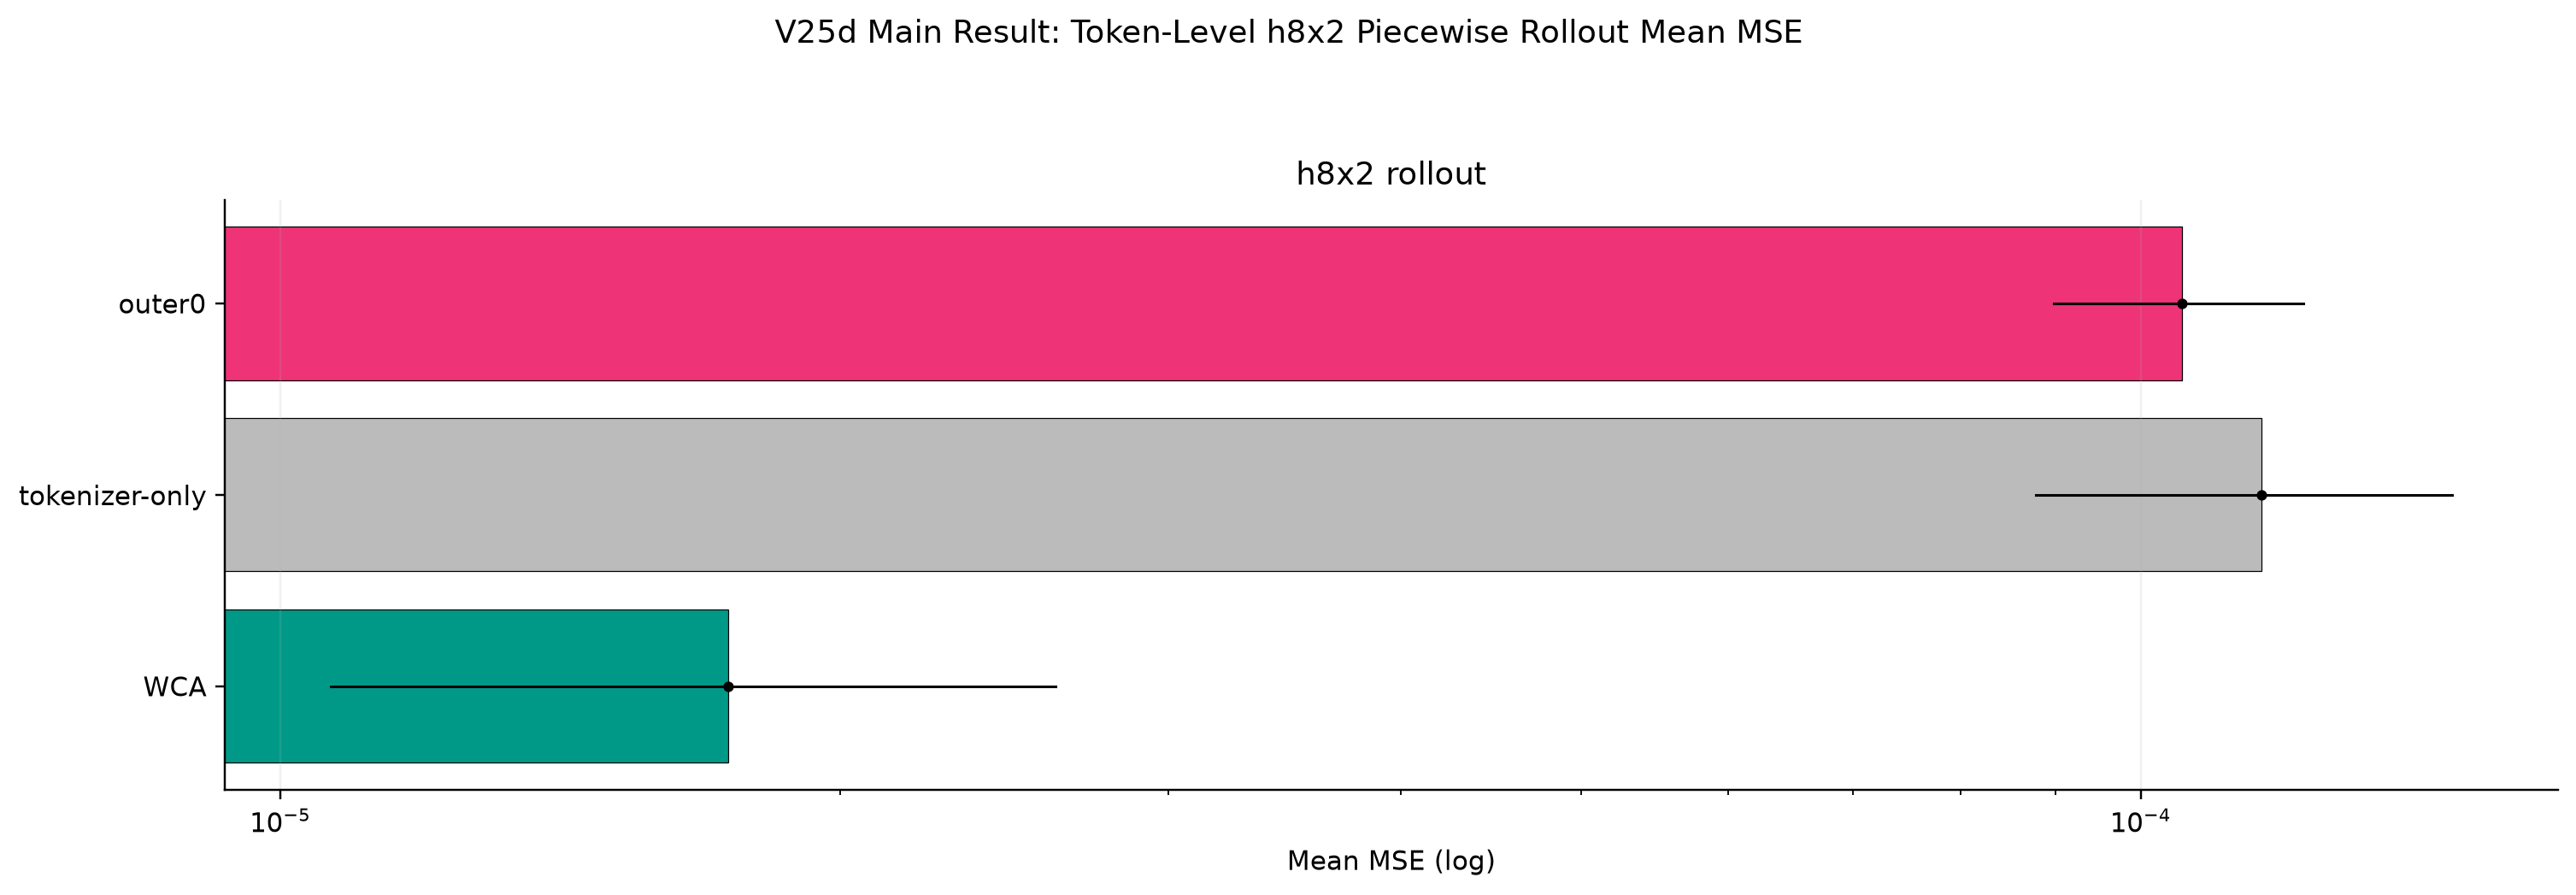
\includegraphics[width=0.86\linewidth]{v25d_rollout_mean_mse.png}
\caption{V25d h8x2 rollout mean MSE. The main formal comparison is
token-level WCA against same-family tokenizer-only and outer0 controls.}
\end{figure}

\begin{figure}[H]
\centering
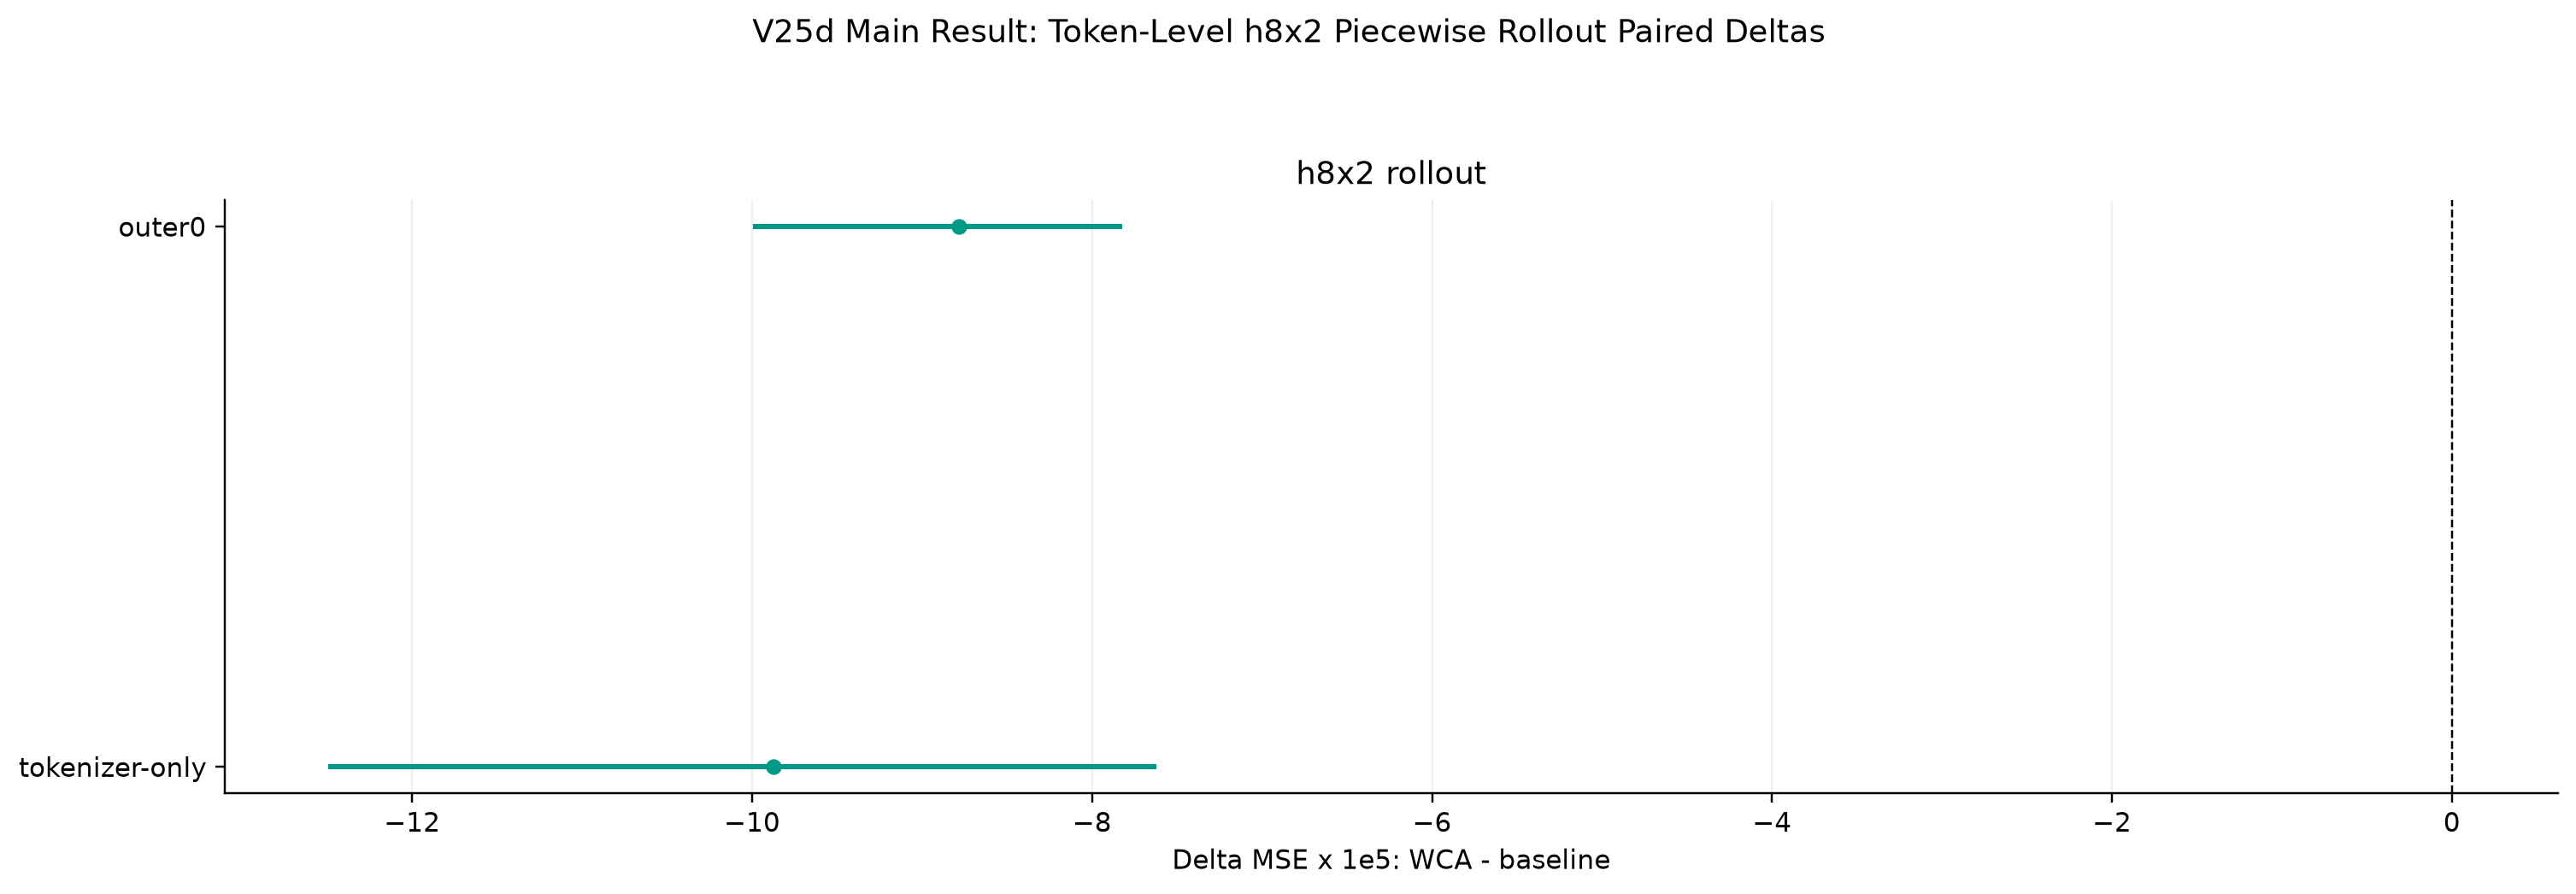
\includegraphics[width=0.86\linewidth]{v25d_rollout_paired_delta.png}
\caption{Paired rollout deltas over fixed starts. This supports the h8x2
token-level rollout claim but does not replace larger multi-seed replication.}
\end{figure}

\section{Qualitative Panels and Metric-Space Boundaries}

The qualitative figures are useful but must be read correctly. WCA token-level
outputs are visualized by repeating predicted patch tokens back into image
patches. This makes the field look blocky by construction. Raw/full-field FNO
or U-Net outputs can preserve within-patch detail. Therefore qualitative panels
show representation boundaries; they do not establish native visual superiority
for WCA.

\begin{figure}[H]
\centering
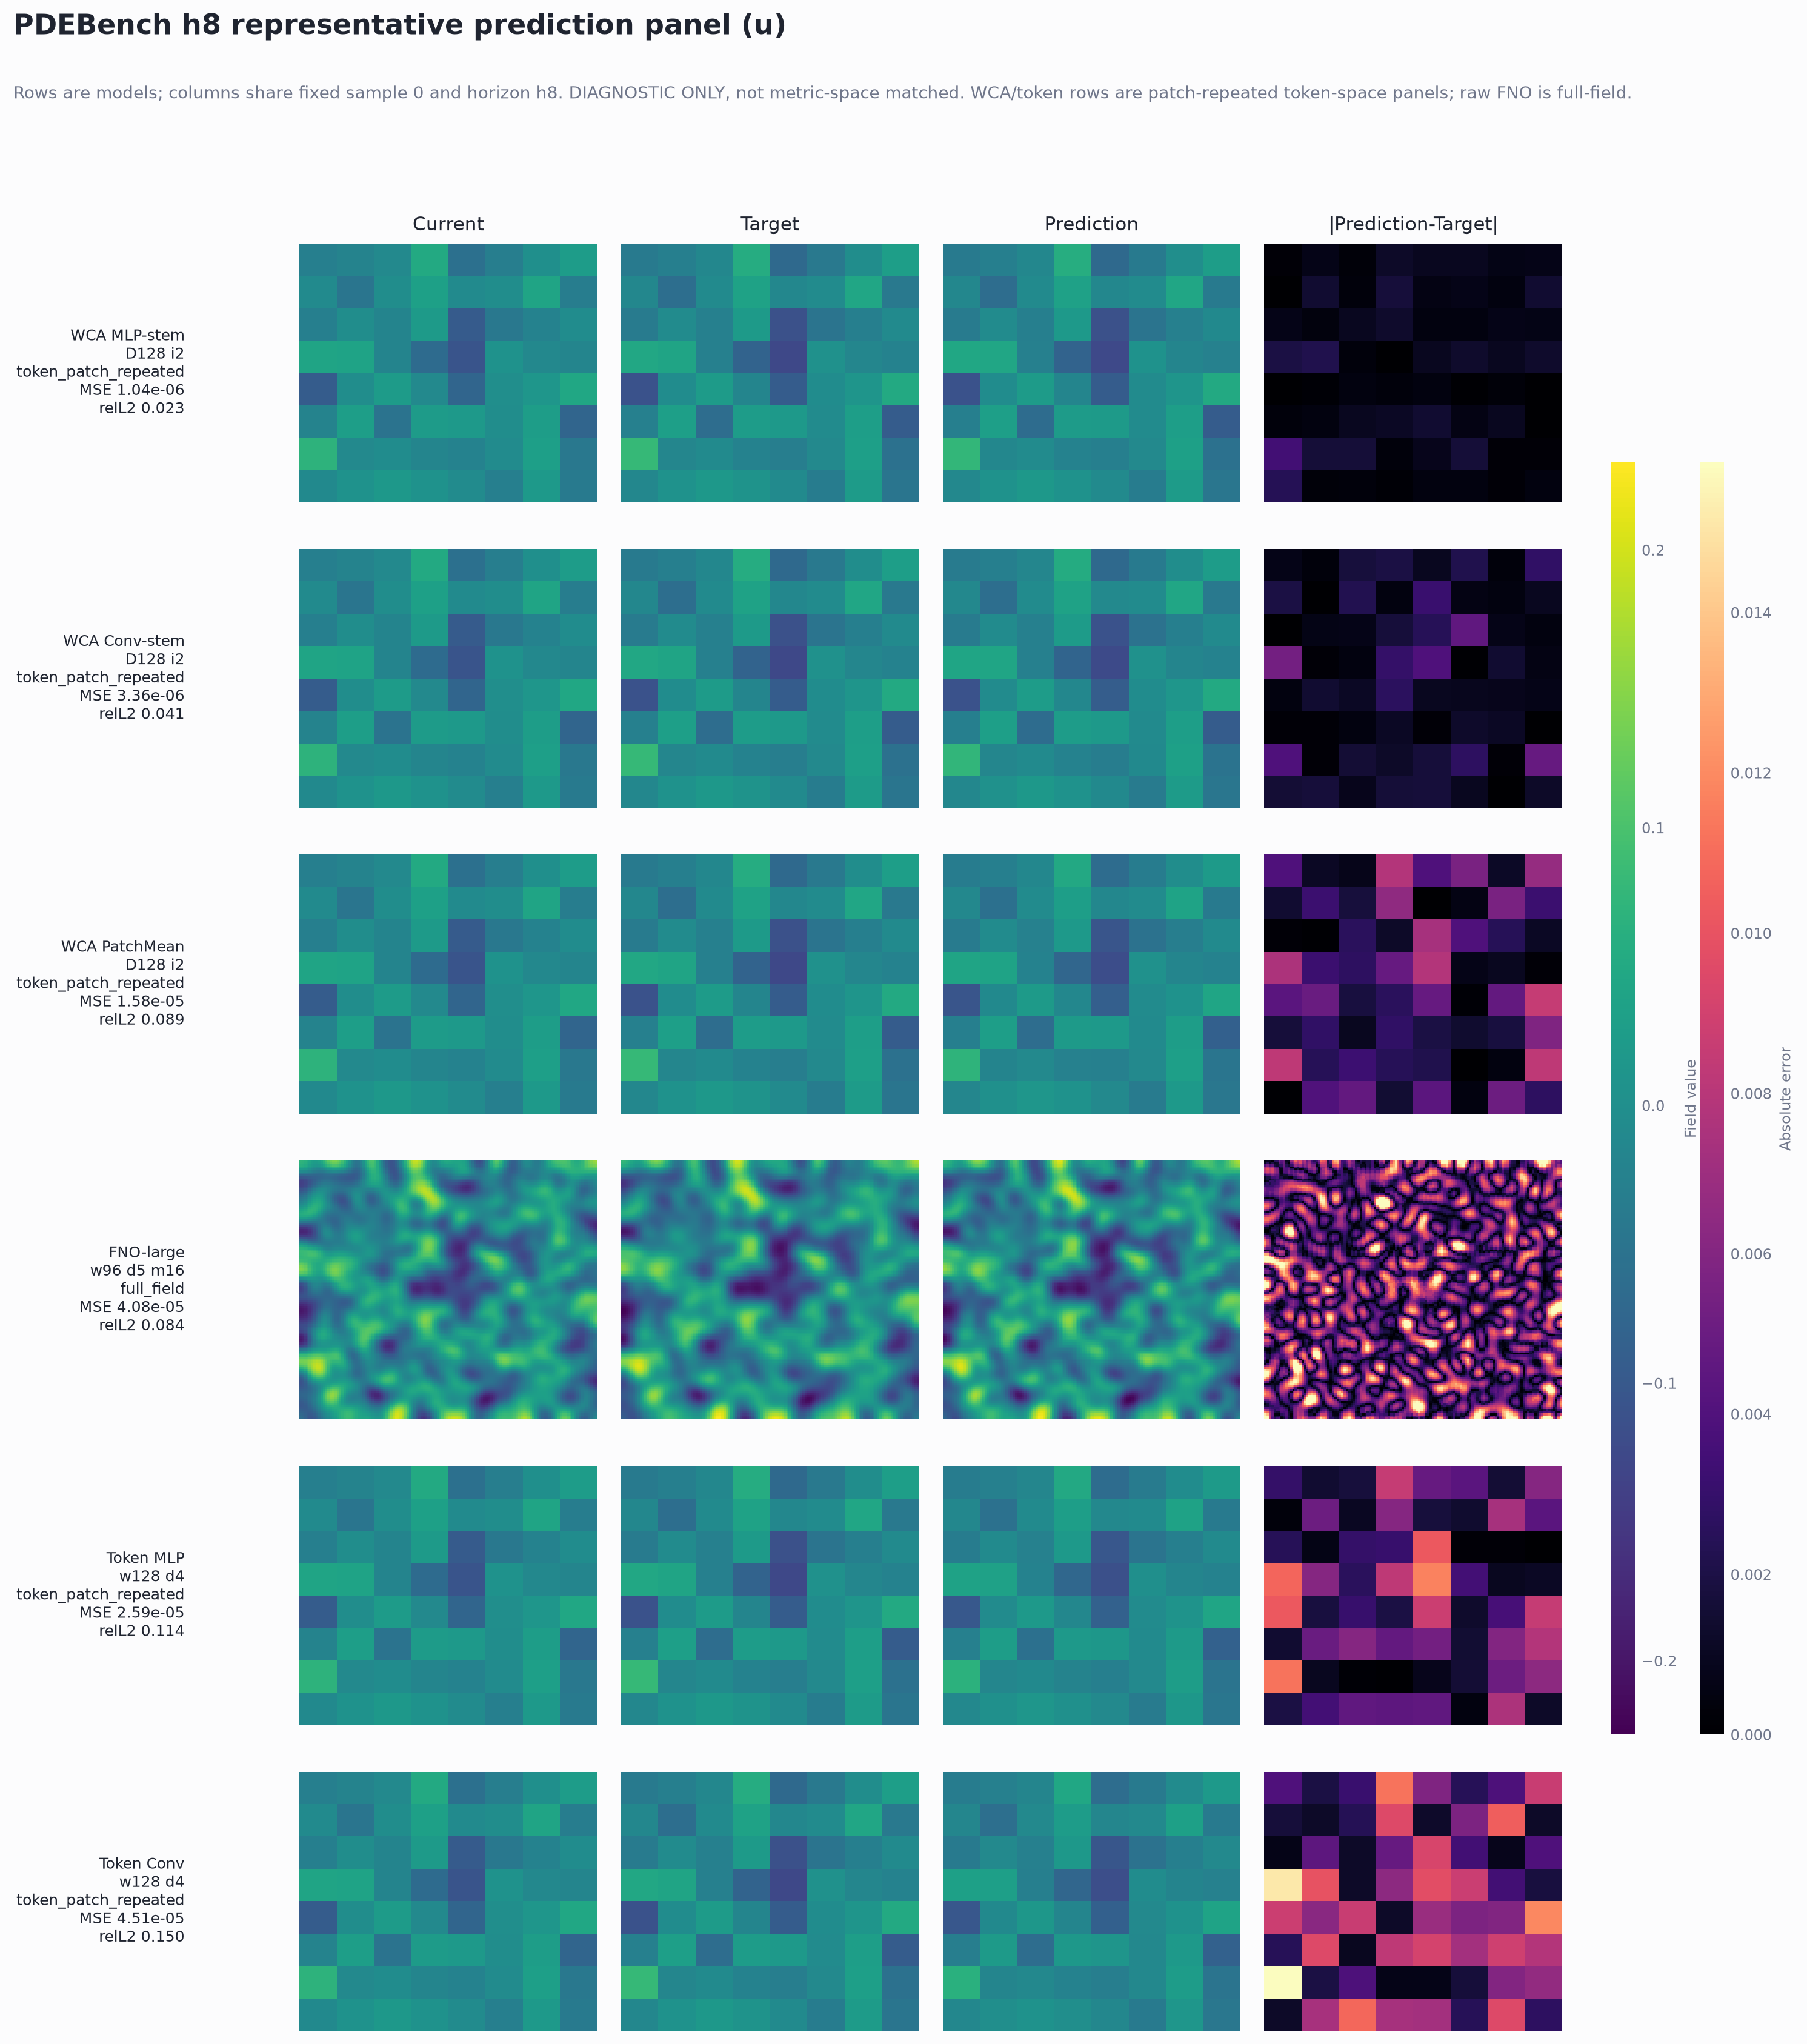
\includegraphics[width=0.95\linewidth]{pdebench_h8_u_model_composite.png}
\caption{PDEBench h8 qualitative panel for channel $u$. WCA/token rows are
patch-repeated token outputs; raw anchors may be full-field outputs.}
\end{figure}

\begin{figure}[H]
\centering
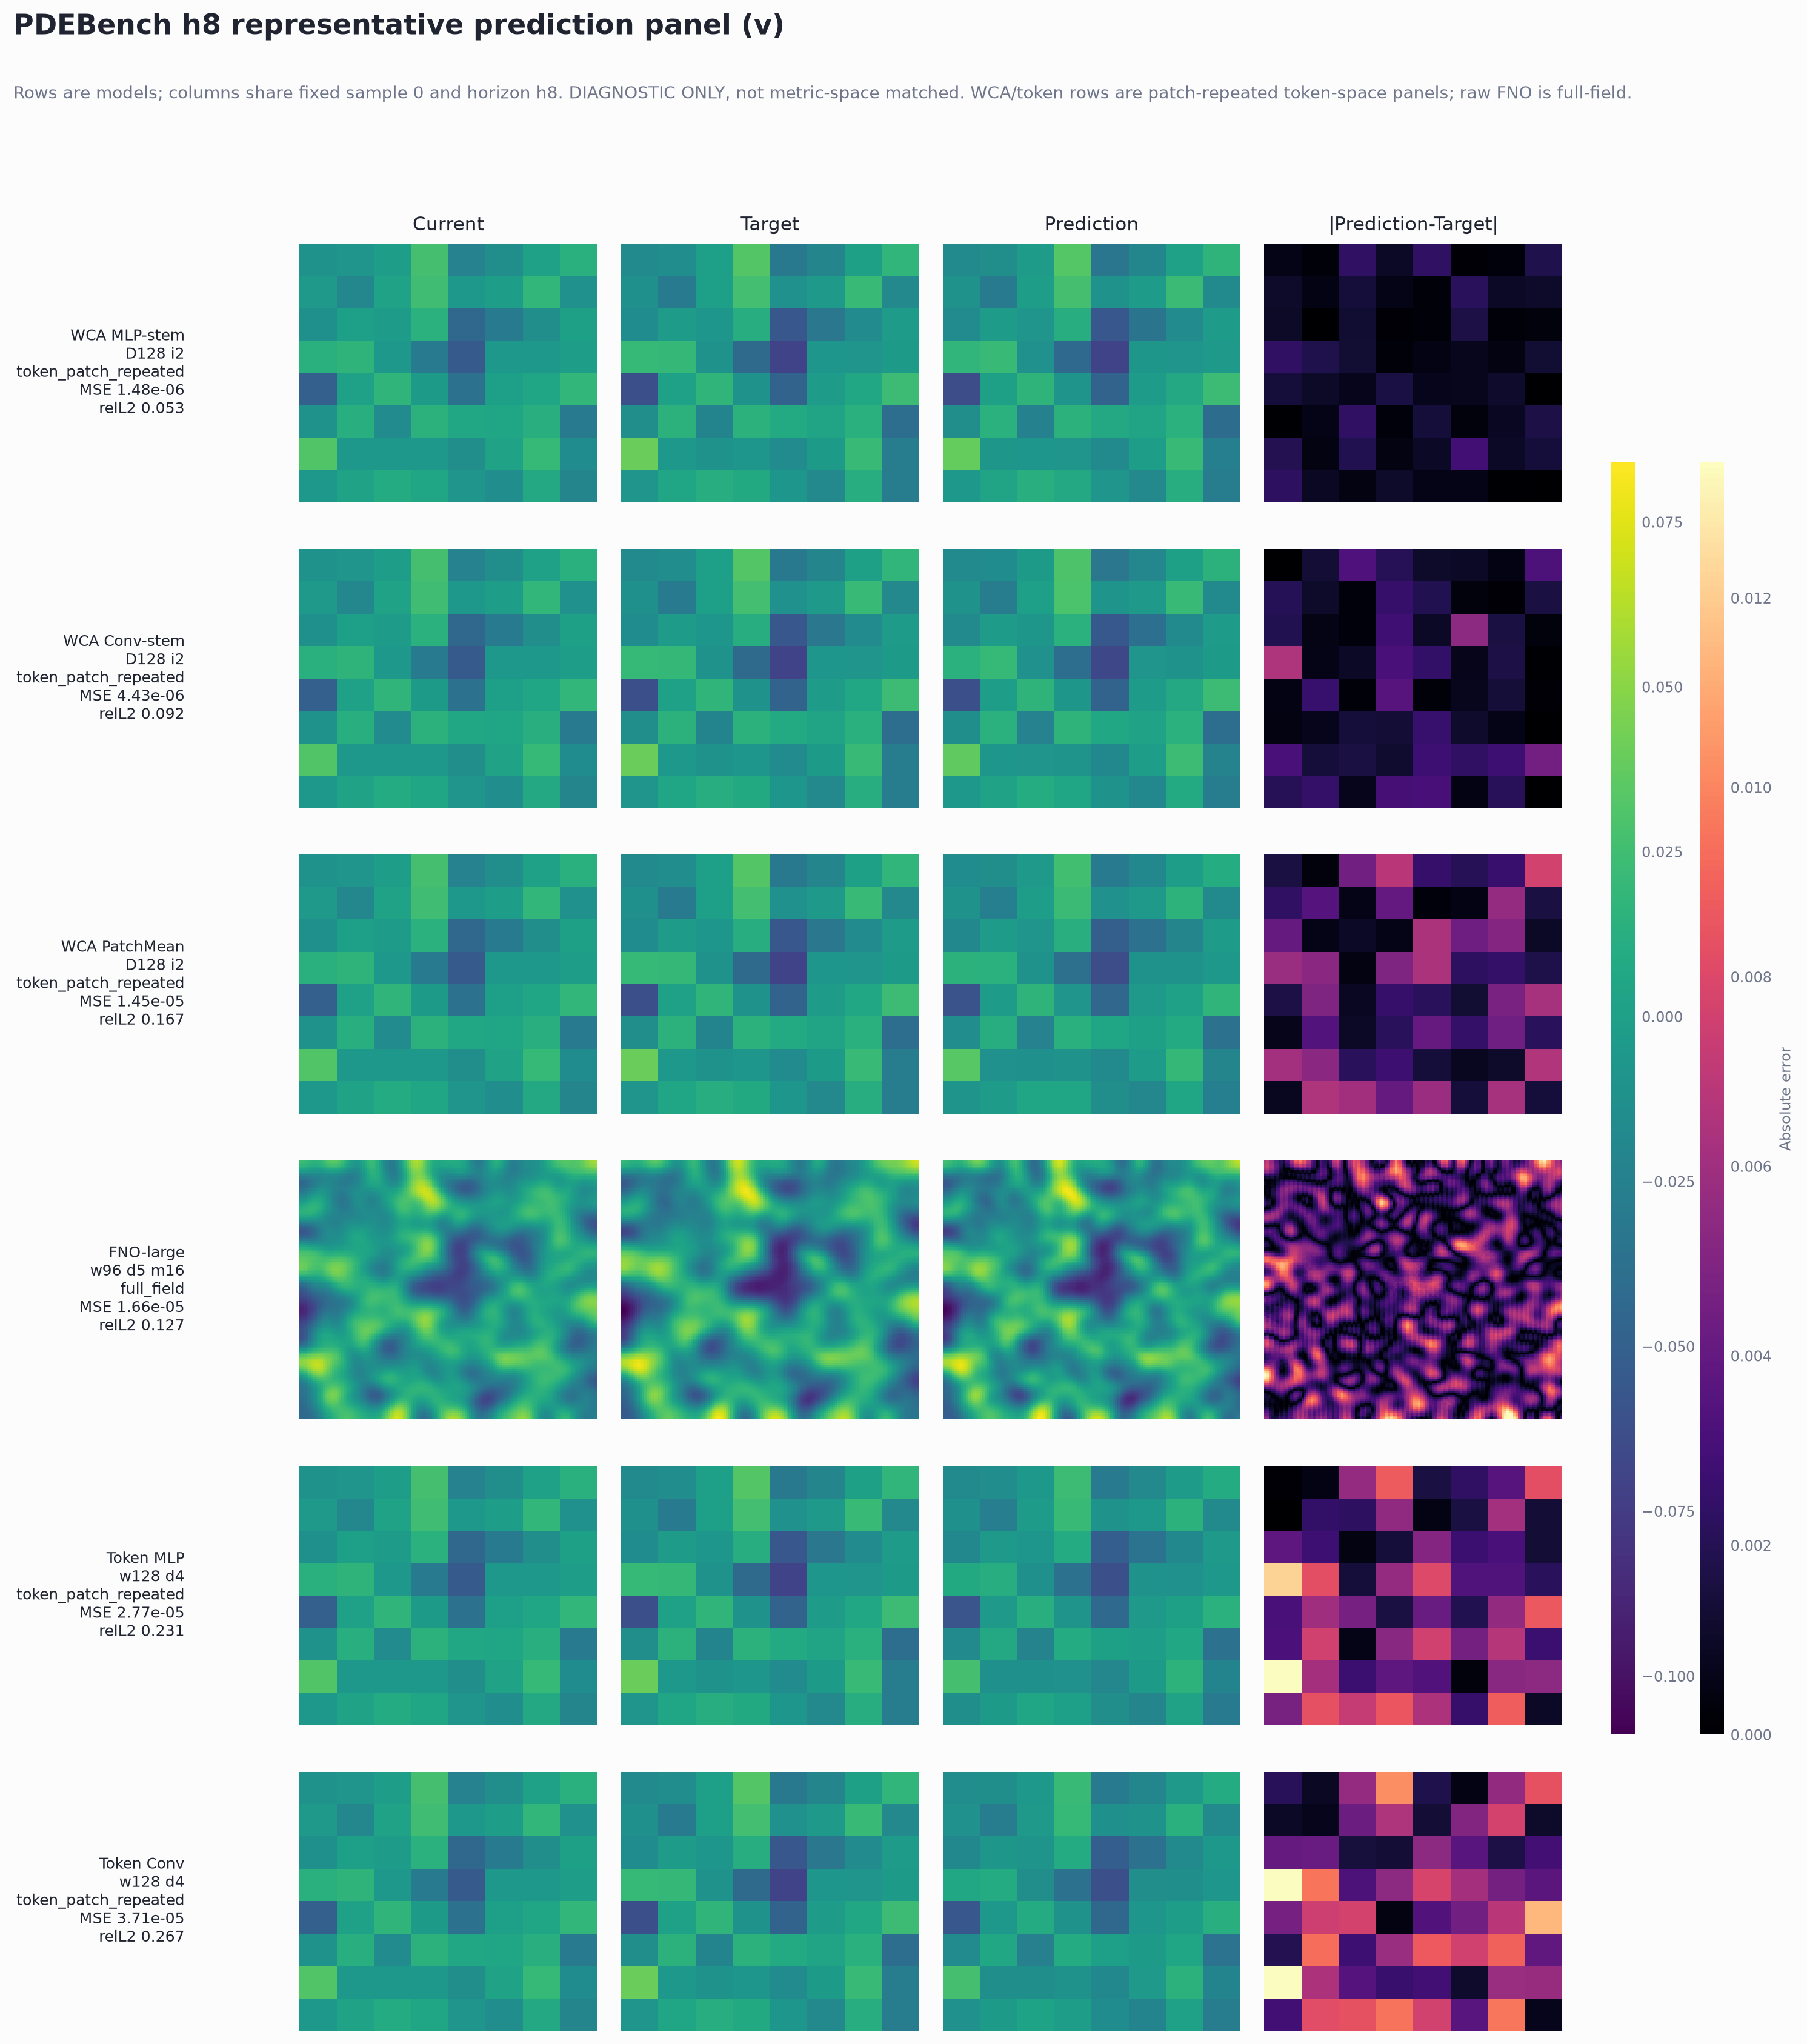
\includegraphics[width=0.95\linewidth]{pdebench_h8_v_model_composite.png}
\caption{PDEBench h8 qualitative panel for channel $v$. Quantitative claims
must come from explicitly declared metric space.}
\end{figure}

\section{Negative Results and Lessons}

Failures are part of the evidence record because they explain which claims are
supported, which ones are not, and where the next experiments should focus.

\subsection{Maze failure modes}

Harder maze families exposed local minima, loops, and shortcut learning. This
means WCA can form useful fields but still needs topology-aware losses and
functional rollout metrics for navigation.

\subsection{PatchMean bottleneck}

PatchMean is auditable but lossy. Its short-horizon weakness helped identify
the need for learnable interfaces. This is a positive scientific outcome:
the interface bottleneck became experimentally visible.

\subsection{N=256 PatchMean boundary}

N=256 PatchMean WCA underperformed matched token baselines. This should not be
read as a theorem that WCA cannot scale. It shows that increasing token count
under a weak interface and dense implementation can expose capacity and
optimization limits. The next scaling test should use learnable interfaces and
capacity-safe recursion ladders.

\subsection{Decoder and tokenizer confounds}

Learnable interfaces improve performance, but they also create attribution
risks. A large decoder can become a model in its own right. The correct
response is not to avoid learnable interfaces; it is to include tokenizer-only,
outer0, decoder-size, and token-equivalent controls.

\section{Current Interpretation}

The current evidence supports four claims.

\begin{enumerate}[leftmargin=2em]
  \item WCA is a coherent architecture distinct from ordinary GNNs, attention,
  and direct neural-operator maps.
  \item Recursion depth matters in the tested PDEBench reaction-diffusion
  setting, especially for h8 under PatchMean.
  \item Learnable interfaces reveal stronger WCA behavior than PatchMean, and
  source-audit controls suggest that the WCA core contributes beyond the
  interface alone on several horizons.
  \item V25d h8x2 token-level rollout provides the cleanest current formal
  evidence that the WCA core can support iterative long-horizon token dynamics.
\end{enumerate}

The current evidence does not finish the research program. The strongest
formal rows are token-level. Native full-field decoding, broader PDE families,
longer rollout, stronger replication, efficient dense-equivalent kernels, and
unified physical latent interfaces remain open.

\section{Roadmap}

\subsection{Native and learnable interfaces}

The next major model direction is a native WCA field interface. The model
should preserve more within-patch information without allowing the decoder to
hide the WCA core. This requires interface ablations, decoder controls, and
token-equivalent baselines.

\subsection{Broader PDE families}

Reaction-diffusion is only one physical family. The next experiments should
include advection, Burgers-type dynamics, wave propagation, diffusion variants,
and Navier-Stokes-like flows when strict split contracts are available.

\subsection{Rollout}

h8x2 is a useful diagnostic, but a stronger world-state test needs longer
rollout, spectrum or energy-drift metrics, native-resolution error, and
stability checks.

\subsection{Efficient dense-equivalent implementation}

Full dense WCA is expensive. The first systems goal is not to change the
mathematics, but to preserve dense semantics while improving memory and GPU
throughput. Later sparse, hybrid, or multiscale variants should be introduced
as explicit variants with equivalence or ablation gates.

\subsection{Unified physical latent}

The long-term direction is a unified physical latent interface. Images,
tactile grids, simulator states, weather fields, maze states, and other
modalities could be encoded into a shared WCA state space. This is a future
branch, not a current result, but it is the natural extension of WCA as a
state-space architecture.

\section{Reproducibility and Release Package}

The public release should include:

\begin{itemize}[leftmargin=2em]
  \item English and Chinese PDF reports;
  \item source LaTeX files and compiled PDFs;
  \item figures and tables used in the report;
  \item a claim table separating formal, source-audit, secondary, diagnostic,
  and future evidence;
  \item artifact manifests with hashes;
  \item GitHub, Hugging Face, and Zenodo release notes;
  \item a reproduction guide that explains the strict split, horizon, token,
  and checkpoint contracts.
\end{itemize}

\section{Conclusion}

World Cellular Automata is a recursive local-world architecture for
world-state modeling. Its defining computation expands a global state into
center-indexed local worlds, evolves those worlds through pair interactions,
and recomposes evolved centers into the next global state. This structure gives
WCA a clear identity: it is not a generic MLP stack, not ordinary graph message
passing, not transformer attention, and not a direct neural operator.

The experiments recorded here show that WCA is worth continued study. Maze
experiments motivate world-field formation and reveal topology failures.
WeatherBench-style runs demonstrate real multivariate field applicability.
PDEBench reaction-diffusion provides the strongest current evidence: recursion
depth matters, learnable interfaces reveal stronger dynamics, and h8x2
token-level rollout supports WCA-core contribution beyond interface-only and
no-recursion controls.

The research program is therefore clear. WCA should be developed as a candidate
world-state modeling primitive, with stricter attribution, stronger native
interfaces, broader physical benchmarks, longer rollout, and efficient
dense-equivalent implementation.

\end{document}
